% =====================================================================
% Section VI -- What Off-Path Staging Does
% SpecAsync-UVM manuscript, draft 1 (2026-11-06)
% Every number: paper/support/RESULTS_FACTS.md Section VI (evidence ids
% in the comments). Platform: RTX 5070 Ti, 595.91.07, kernel 7.0.0-34,
% our module (E0.9b/E1: 5997D238; E4-E6: 33FD42E6). Stencil-24K and
% GraphBFS-23 throughout.
% [CALC] marks a value I derived from extract values (ratio, share);
%        have Claude Code recompute before submission.
% [FIG]  figure file names from RESULTS_FACTS VII(f); confirm paths.
% =====================================================================

\section{What Off-Path Staging Does}
\label{sec:spec}
\label{sec:squeeze}

This section reports the speculation results, organised around the two
channels of Section~\ref{sec:bg-where}: the copy inside D5, and the count in
the density rule. Every comparison is against the configurations of
Table~\ref{tab:configs}; C0, the shipped driver, is the comparison of record.

\subsection{Without the Prefetcher: Copy Offload, No Fewer Faults}
\label{sec:spec-off}

With the prefetcher off, the oracle at full width (C6-W512) stages ahead of
demand 99.95\% of the 1{,}125{,}000 distinct pages of Stencil-24K
(\texttt{E4.mech.stencil.C6-W512}). Demand faults do not fall: 2{,}960{,}758,
against 2{,}921{,}620 with speculation off (C1), 1.3\% more
(\texttt{E4.mech.stencil.C1}). This is Section~\ref{sec:bg-resident-mapped}
observed: a staged page is resident, but still unmapped, so the GPU faults on
it anyway.

The faults become cheaper. Stencil-24K runs 23.29\% faster than C1 at
$W = 512$ and 21.62\% faster at $W = 64$ (\texttt{E4.F3.stencil.C6-W512\_vs\_C1},
\texttt{-W64\_vs\_C1}); at $W = 1$ the gain is 9.69\%, because the queue
overflows and drops 318{,}820 of its predictions
(\texttt{E4.mech.stencil.C6-W1}). The phase decomposition, taken for the
earlier one-page configuration with the original lookup (C6-L4096, E1), shows
where such a gain comes from: the dispatch phase D5 falls from 1.60\,s to
0.91\,s per run, since much of the copy it would have issued has already been
made, while the time the servicing thread spends before taking the lock, in the
prediction hook, rises by 0.48\,s (\texttt{E1PartB.stencil.D5}, \texttt{E1b.stencil.C64096-C1}). On
GraphBFS-23, whose oracle is weaker, the gain is under 1\%
(\texttt{E4.F3.graphbfs.C6-W512\_vs\_C1}).

None of this approaches the shipped driver. C6-W512 is $2.92\times$ slower than
C0 on Stencil-24K (\texttt{E4.F4.stencil.C6-W512\_vs\_C0}) and 3.86\% slower on
GraphBFS-23. The prefetcher prevents most faults; staging prevents none, so
turning the prefetcher off to make room for staging costs far more than staging
recovers. In what follows, C1 is used only to isolate this copy-offload
channel.

\subsection{With the Prefetcher: A Gain, Through the Density Rule}
\label{sec:spec-on}

With the prefetcher on at its shipped threshold, the full-width oracle (C7-W512)
beats the shipped driver on Stencil-24K in each of three independent sessions:
by 4.93\% in E4, 5.26\% in E5 and 3.36\% in E6 (\texttt{E4.F1.stencil.C7-W512\_vs\_C0},
\texttt{E5.wall.t51}, \texttt{E6.F1.C7W512-t51\_vs\_C0-t51}). The E4 result
fired that gate's pre-registered falsification trigger, which had been written
to detect exactly this outcome, and reversed this study's earlier conclusion
(Section~\ref{sec:pitfalls}). Width matters: at $W = 1$ the oracle is 5.87\%
\emph{slower} than C0, and at $W = 64$ the difference is not significant
(\texttt{E4.F1.stencil.C7-W1\_vs\_C0}, \texttt{-W64\_vs\_C0}). On GraphBFS-23 no
width differs detectably from C0; at $W = 512$ the difference is $-0.06\%$
against a minimum detectable effect of 0.38\% at the family's level
(\texttt{E4.F1.graphbfs.C7-W512\_vs\_C0}, \texttt{E4.mde\_family.graphbfs.F1}).

The gain is not the copy offload of Section~\ref{sec:spec-off}. With the
prefetcher on, the worker finishes first for only 2.07\% of distinct pages
(\texttt{E5.mech.t51.C7W512}), yet demand faults fall from 339{,}386 to
203{,}331, a 40.1\% reduction (\texttt{E5.D(51)}). Section~\ref{sec:bg-prefetcher}
predicts how: staged pages count toward the density rule, so regions pass the
threshold sooner, and the prefetcher maps them during ordinary fault service.

E5 tested this explanation with a pre-registered dose--response rule
(Section~\ref{sec:protocol}). If staging acts through the density rule, its
fault reduction $D(t)$ should be larger at a higher threshold, where the rule
needs more counted pages, and should vanish when the rule cannot pass. It did
both. $D$ rose to 53.4\% at threshold 75 (\texttt{E5.D(75)}). At threshold 100,
where the strict test of (\ref{eq:density}) can never pass, $D$ was $-2.2\%$:
staging slightly increased demand faults (\texttt{E5.D(100)}), and the verdict rule returned \emph{Supported}. The
wall-clock gains follow the same order, 5.26\%, 10.12\% and 21.04\% at 51, 75
and 100 (\texttt{E5.wall.t51}, \texttt{t75}, \texttt{t100}); at 100 the gain is
copy offload alone, as in Section~\ref{sec:spec-off}, and the configuration is
still far slower than C0.

\begin{figure}[t]
\centering
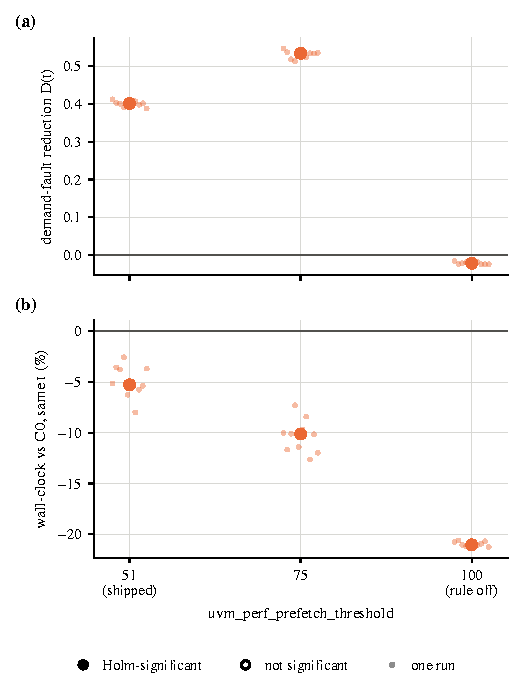
\includegraphics[width=\columnwidth]{figures/fig_e5_threshold_dose_response}
\caption{Fault reduction from staging grows with the threshold and vanishes
when the density rule is disabled (E5, Stencil-24K, C7-W512 vs C0 at each
threshold; 10 runs per cell).}
\label{fig:e5}
\end{figure}

\subsection{The Same Lever Without Speculation}
\label{sec:spec-matched}

If staging gains only by helping regions pass the threshold, lowering the
threshold should gain at least as much without staging. E6 tested this with a
second pre-registered trigger: it would fire if any stock configuration at a
lower threshold was not significantly slower than C7-W512 at 51. It fired. C0 at
threshold 0 is faster than C7-W512 at 51, which is 6.39\% slower than it; at
threshold 10 the oracle is 4.72\% slower, and at 25 the two do not differ
detectably (\texttt{E6.F1.C7W512-t51\_vs\_C0-t0}, \texttt{-t10}, \texttt{-t25}).

At matched thresholds, speculation adds little. Its gain is $-0.85\%$ at
threshold 0 and $-0.28\%$ at 10, neither significant, against minimum detectable
effects of 2.04\% and 2.28\% at the family's level, and 2.76\% at 25, which is
significant (\texttt{E6.wall.C7W512-t0\_vs\_C0-t0}, \texttt{-t10}, \texttt{-t25},
\texttt{E6.mde\_family.stencil\_wall}). Staging still removes faults at every
threshold, 5.3\% of them at 0 and 22.1\% at 25 (\texttt{E6.demand.*}), but at low
thresholds the prefetcher has already taken most regions, and the faults that
remain are too few to matter: one pre-registered expectation predicted a
wall-clock gain from the 5.3\% at threshold 0, and it failed (X4).

\begin{figure}[t]
\centering
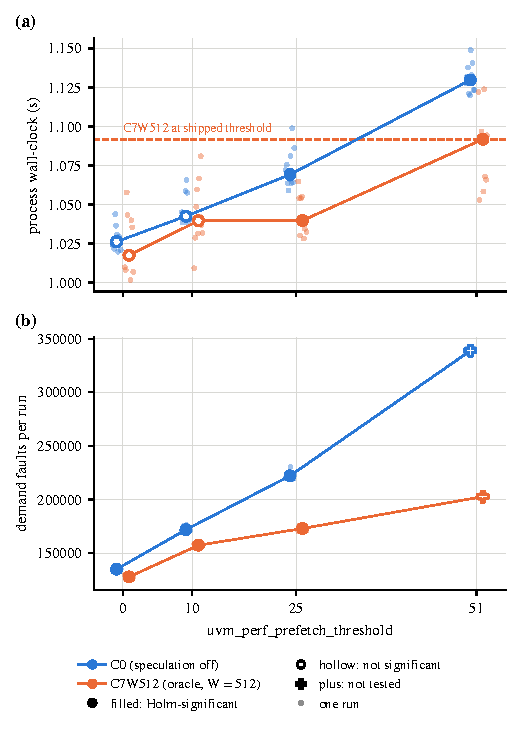
\includegraphics[width=\columnwidth]{figures/fig_e6_threshold_baseline}
\caption{C7-W512 at the shipped threshold against the stock driver at lower
thresholds, and each threshold with and without speculation (E6, Stencil-24K).}
\label{fig:e6}
\end{figure}

\subsection{What Speculation Costs on the Critical Path}
\label{sec:spec-cost}

The prediction hook runs on the servicing thread for every fault. Handing one
prediction to the worker costs 54\,ns with the prefetcher off and 75\,ns with it
on, on Stencil-24K, and 114\,ns on GraphBFS-23
(\texttt{E1b.stencil.C64096-C1}, \texttt{E1b.stencil.C74096-C0},
\texttt{E1b.graphbfs.C64096-C1}). With the original oracle the rest of the hook,
the lookup itself, cost a further 140--167\,ns per fault. The fast lookup of
Section~\ref{sec:design-oracle} removed 78--88\% of that residual
(\texttt{E3b.*.residual}): an instrument meant to bound speculation had been
paying most of speculation's per-fault cost itself (catalog entry~21).

At full width the queue is never the bottleneck: C7-W512 enqueues about 2{,}200
items per Stencil-24K run and drops none (\texttt{E4.mech.stencil.C7-W512}).

\subsection{Summary}

Off-path staging, driven by an oracle as good as the workload allows, does two
things in this driver. It moves copy work off the servicing thread, which is
worth 21--23\% only against a driver whose prefetcher is off, and it feeds the
prefetcher's density count, which is
worth 3.4--5.3\% against the shipped driver.
It prevents no fault directly. The second effect is available, and larger,
from the threshold alone; Section~\ref{sec:threshold} measures what that lever
does on its own.
